% Created 2018-02-06 Tue 15:09
\documentclass[11pt]{article}
\usepackage[utf8]{inputenc}
\usepackage[T1]{fontenc}
\usepackage{fixltx2e}
\usepackage{graphicx}
\usepackage{longtable}
\usepackage{float}
\usepackage{wrapfig}
\usepackage{rotating}
\usepackage[normalem]{ulem}
\usepackage{amsmath}
\usepackage{textcomp}
\usepackage{marvosym}
\usepackage{wasysym}
\usepackage{amssymb}
\usepackage{hyperref}
\tolerance=1000
\usepackage[hyperref,x11names]{xcolor}
\usepackage{amsmath}
\date{\today}
\title{Report}
\hypersetup{
  pdfkeywords={},
  pdfsubject={},
  pdfcreator={Emacs 25.2.2 (Org mode 8.2.10)}}
\begin{document}

\maketitle
\tableofcontents




\section{Check list}
\label{sec-1}
\begin{itemize}
\item $\boxtimes$ Do not round the state value to grids.
\item $\boxtimes$ Change the action of buying client capital from increments to choosing the exact value.
\item $\boxtimes$ Remove the depreciation factor and use an upper bound on the possible client capital.
\item $\square$ Make sure the action of quality > 0 when client capital >0: the firm must produce 
something when they are in the (have entered or being entering) the game.
\item $\boxtimes$ Change the cost of choosing a client capital value,
\begin{itemize}
\item $\boxtimes$ If k == 0 and k' > 0: pay a entry cost. The total cost will be 
"client capital price*(k'-k) + entry cost"
\item $\boxtimes$ If k \texttt{= 0 and k' =} 0: total cost=0
\item $\boxtimes$ If k > 0 and k' > k: total cost = client capital price*(k'-k) + maintenance cost*k.
\item $\boxtimes$ If k > 0 and k > k' > 0: total cost = -sale price*(k-k') + maintenance cost*k'.
\item $\boxtimes$ If k > 0 and k' == 0: obtain a scrap value. total cost = -sale price*k - scrap value.
\end{itemize}
\item $\boxtimes$ Make sure that if client capital is 0, the cost to produce a nonzero quality product 
is infinity. (Use 30 penalty as infinity)
\item $\square$ Also, try to add a 0-profit constraint on actions, that is: enforce each firm must 
have nonnegative stage pay off at any stage.
\end{itemize}

\section{The Model}
\label{sec-2}
\subsection{Basic parameters}
\label{sec-2-1}
\begin{center}
\begin{tabular}{|l|r|}
\hline
Entry cost & 0.03\\
Client capital unit price & 0.005\\
Maintenance unit cost & 0.005\\
Scrap value & 0.01\\
Unit production cost & 0.01\\
Number of normals & 36\\
\hline
\end{tabular}
\end{center}

\subsection{Grids}
\label{sec-2-2}
\begin{center}
\begin{tabular}{|l|r|}
\hline
State & 0:1:5\\
Action of client capital & 0:1:5\\
Action of quality & 0:1:5\\
Action of price & 0:1:5\\
\hline
\end{tabular}
\end{center}

\subsection{Equations}
\label{sec-2-3}
\begin{itemize}
\item Setup cost
\end{itemize}
\[ C_{s}=\begin{cases} 0 & w=0 \\ \frac{w^2}{20a} & w\ne0, k > 0 \\ 30 & w\ne0, k=0 \end{cases}\]

\section{Results}
\label{sec-3}
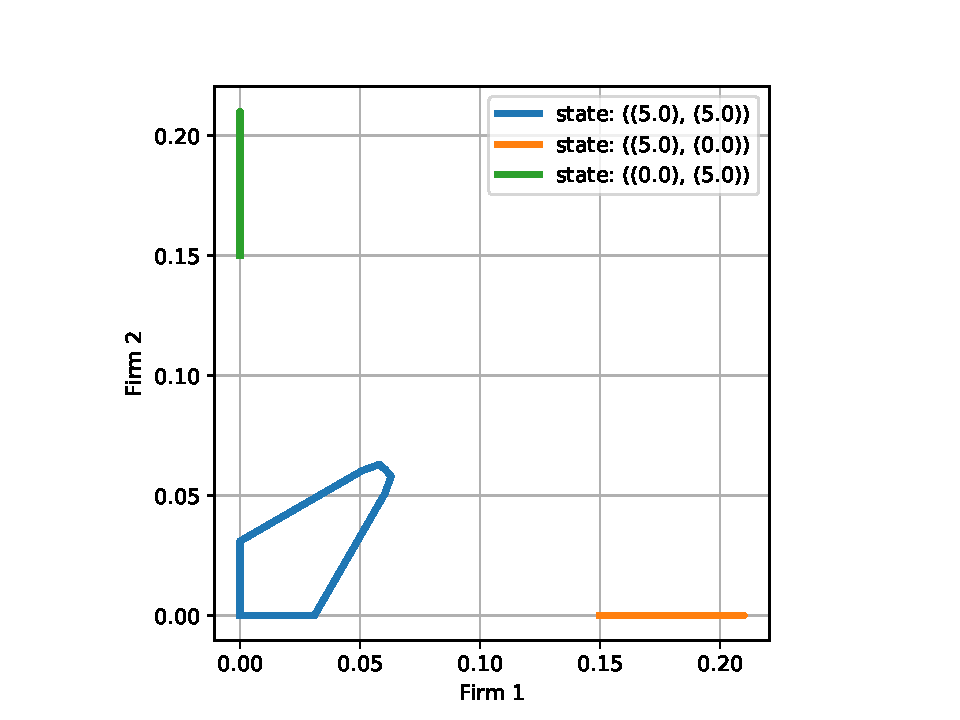
\includegraphics[width=.9\linewidth]{./img/overlap_35_30_5.pdf}

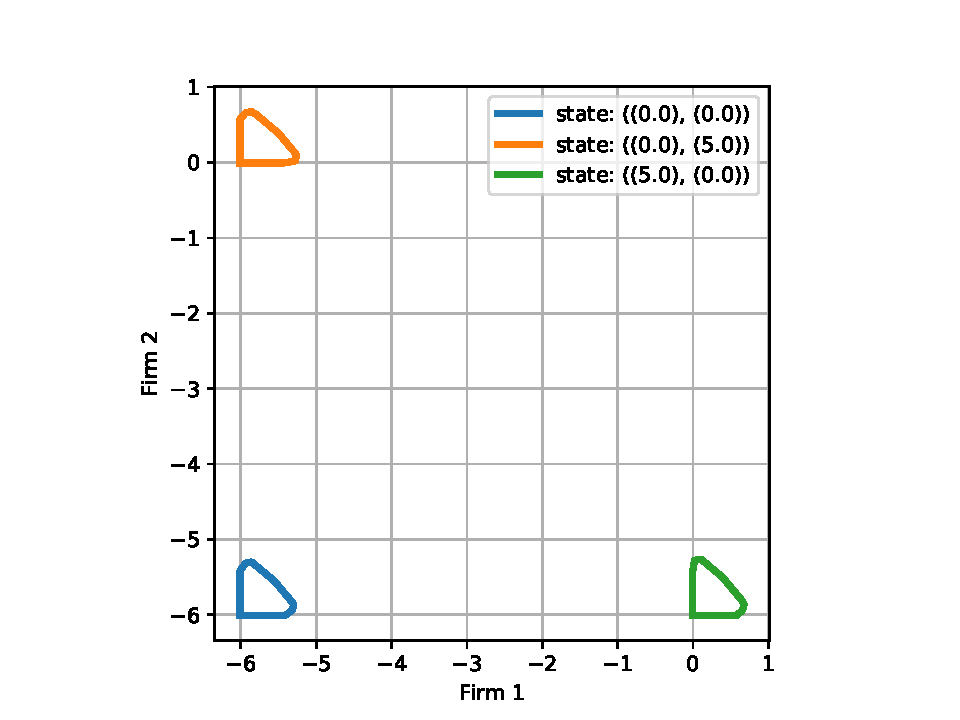
\includegraphics[width=.9\linewidth]{./img/overlap_0_5_30.pdf} 

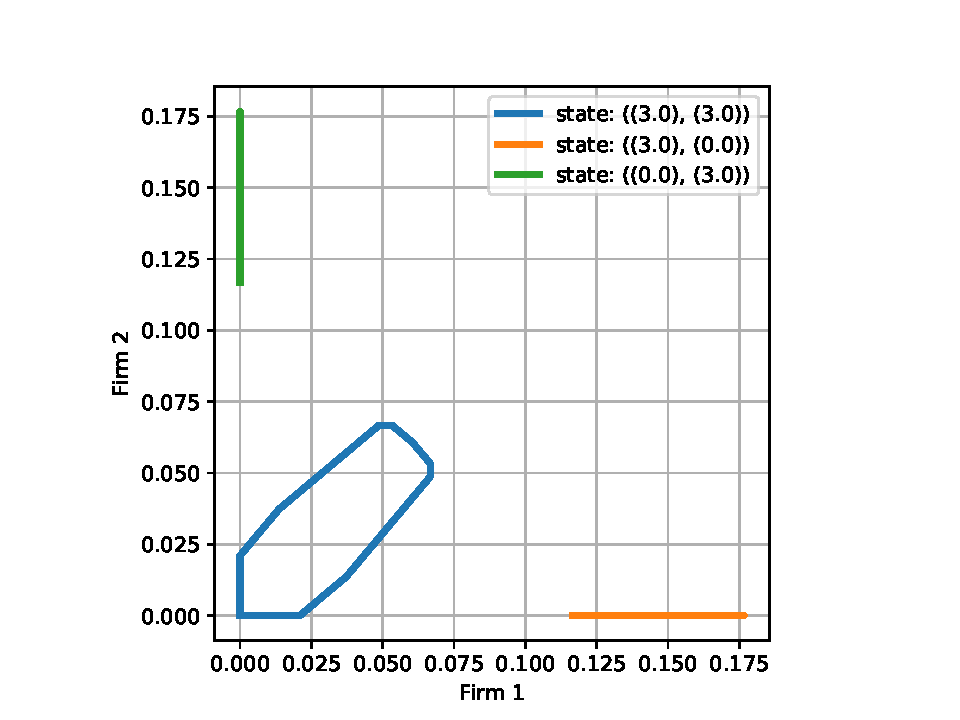
\includegraphics[width=.9\linewidth]{./img/overlap_21_18_3.pdf}

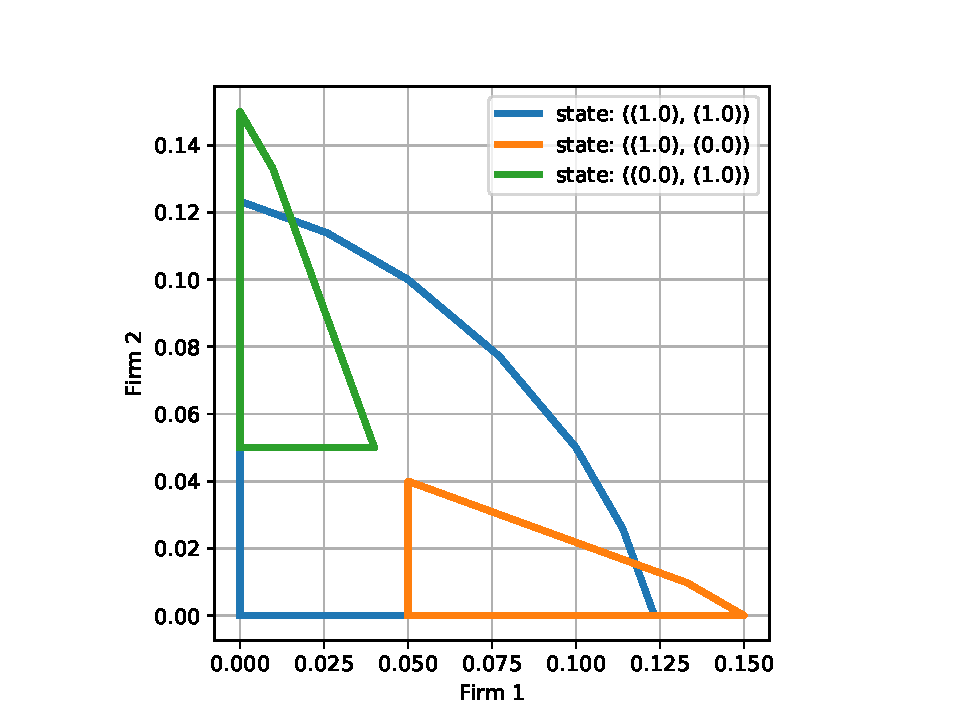
\includegraphics[width=.9\linewidth]{./img/overlap_7_6_1.pdf}

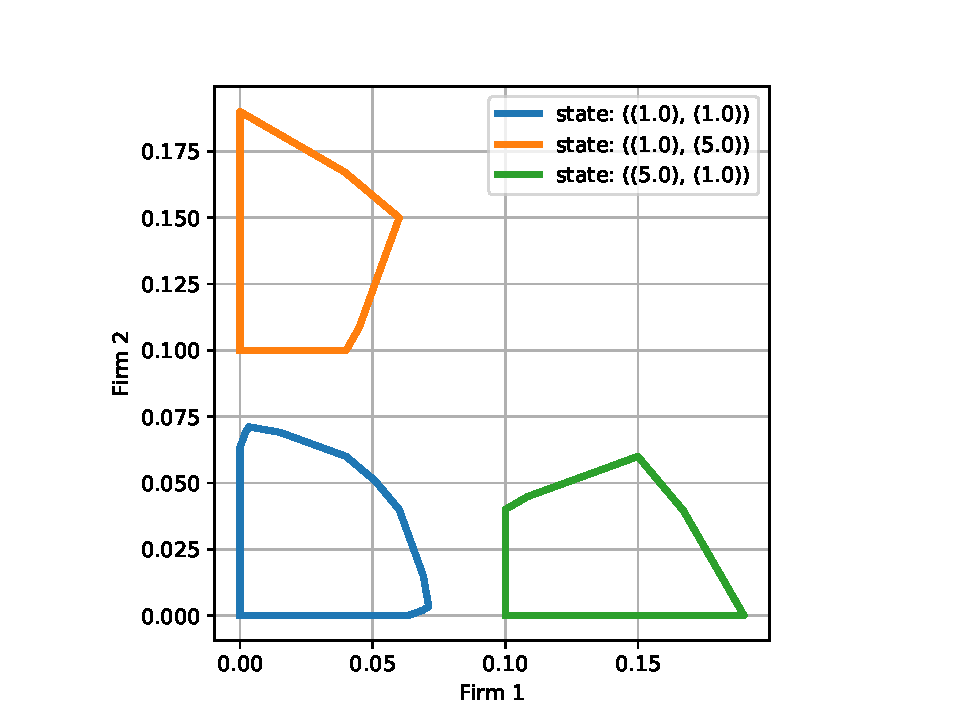
\includegraphics[width=.9\linewidth]{./img/overlap_7_11_31.pdf}

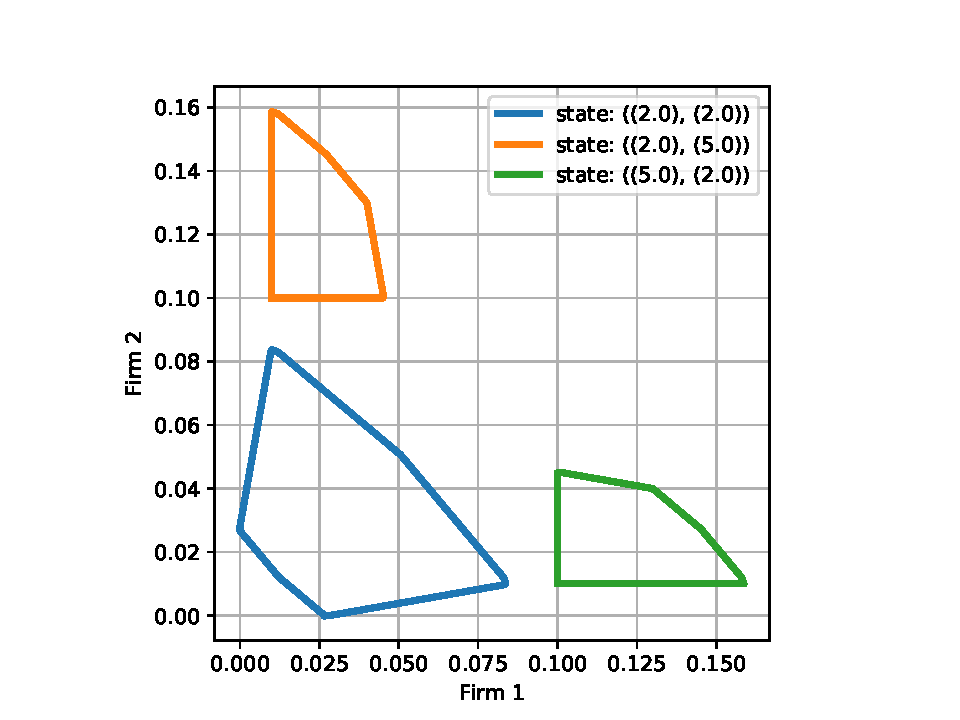
\includegraphics[width=.9\linewidth]{./img/overlap_14_17_32.pdf}

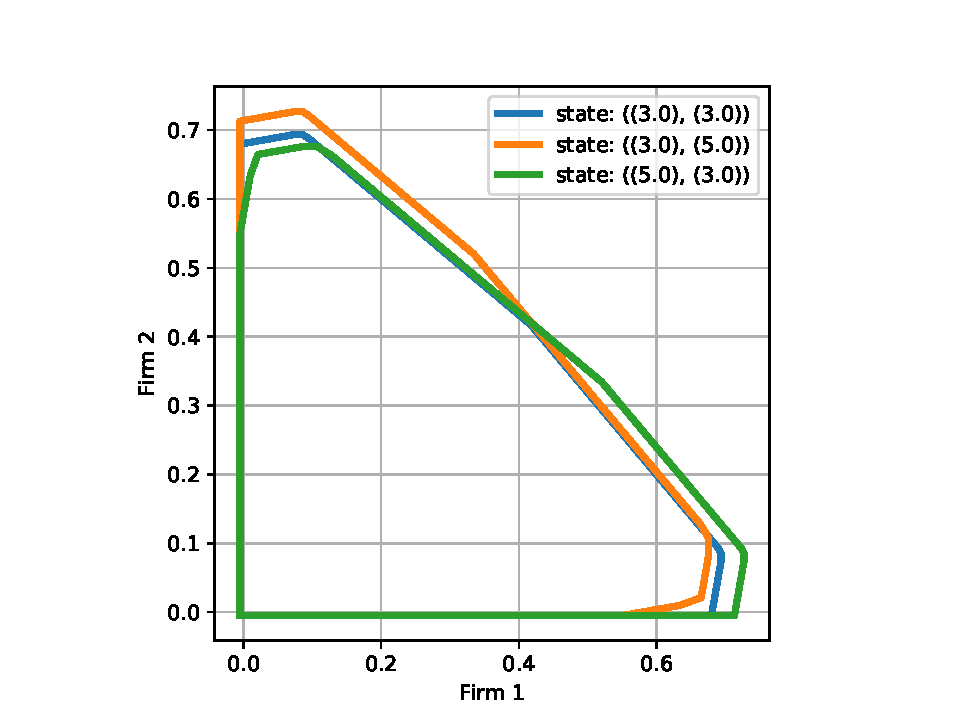
\includegraphics[width=.9\linewidth]{./img/overlap_21_23_33.pdf}

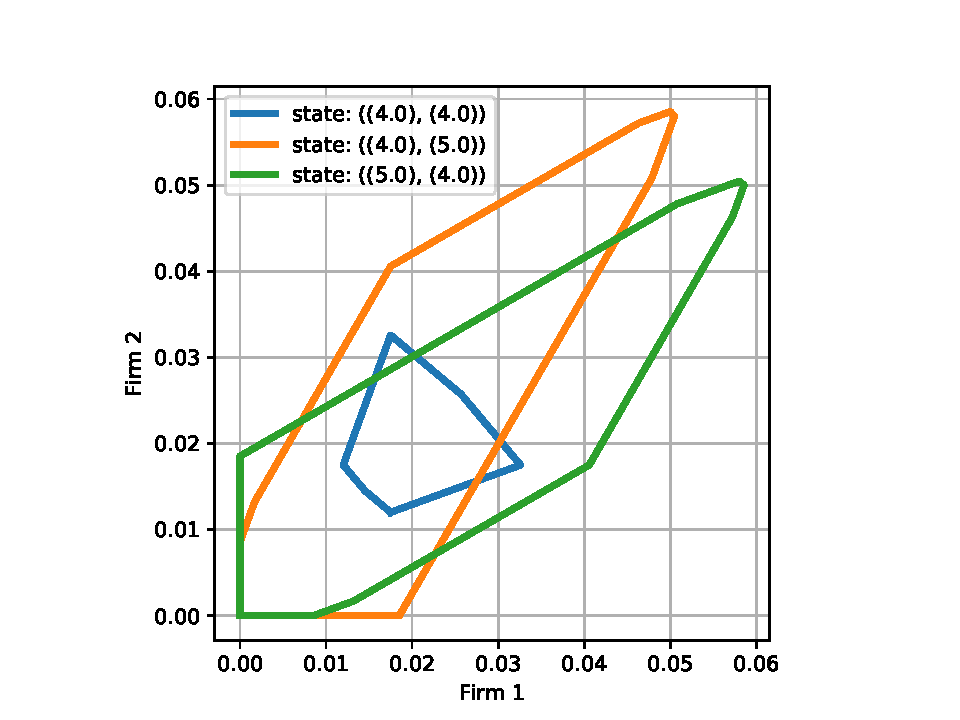
\includegraphics[width=.9\linewidth]{./img/overlap_28_29_34.pdf}
% Emacs 25.2.2 (Org mode 8.2.10)
\end{document}